\def\makemunitresults{
    \section{Kết quả của mô hình MUNIT}
    
    \subsection{Các bộ dữ liệu}
    \subsubsection{Bộ dữ liệu Edges and shoes/handbags}
    Edges and shoes/handbags\index{edges and shoes/handbags} là bộ dữ liệu bao gồm hình ảnh của các đôi giày và túi xách và các hình ảnh viền cạnh được sinh ra bởi Holistically-Nested Edge Detection. Tuy nhiên, MUNIT không luyện với các cặp dữ liệu có sẵn mà chỉ sử dụng hai nhóm ảnh: ảnh thật và ảnh đường nét.

    \subsubsection{Bộ dữ liệu Animal image translation}
    Animal image translation là bộ dữ liệu gồm 3 domain là mèo nhà, mèo hoang và chó. MUNIT được huấn luyện độc lập với mỗi một cặp domain khác nhau.

    \subsubsection{Bộ dữ liệu Street scene images}
    MUNIT được thử nghiệm với hai bộ dữ liệu con:
    \begin{itemize}[leftmargin=0cm,itemindent=.5cm,labelwidth=\itemindent,labelsep=0cm,align=left]
    \item \textbf{Bộ dữ liệu Synthetic and real:} Tác giả sử dụng ảnh đường phố được dựng lại từ bộ dữ liệu SYNTHIA và ảnh đường phố được chụp thật từ bộ dữ liệu Cityscape. Các ảnh được lấy với mùa, thời tiết và điều kiện ánh sáng khác nhau.
    \item \textbf{Bộ dữ liệu  Summer and winter:} Tác giả sử dụng những ảnh đường phố từ các video hành trình vào mùa hạ và mùa đông. 
    \end{itemize}

    \subsubsection{Bộ dữ liệu Yosemite summer and winter (HD)}
    Yosemite summer and winter (HD) là bộ dữ liệu bao gồm 3253 ảnh mùa hạ và 2385 ảnh mùa đông của Yosemite. Tất cả các ảnh đều là ảnh chất lượng cao và được thay đổi kích thước cạnh nhỏ hơn về 1024 pixel và giữ nguyên tỉ lệ.
    
    \subsubsection{Bộ dữ liệu CelebA-HQ}
    CelebA-HQ là phân bản chất lượng cao của bộ dữ liệu CelebA \cite{celeba}. CelebA-HQ là bộ dữ liệu gồm 30,000 ảnh chân dung khuôn mặt của người nổi tiếng với kích thước 1024x1024 pixel. Ảnh của bộ dữ liệu được chia thành các class gồm các thuộc tính của khuôn mặt. Trong thử nghiệm này, ta chỉ sử dụng ảnh thuộc 2 lớp nam và nữ để thực hiện bài toán Image-to-Image Translation.
    
    \subsection{Lập trình mô hình}
    Code của lập trình mô hình MUNIT được nhóm tác giả cung cấp tại \\ https://github.com/NVlabs/MUNIT. Một số đoạn code quan trọng được tổng hợp tại phần Phụ lục của đồ án.
    
    \subsection{Các phương pháp đánh giá mô hình}
    \subsubsection{Đánh giá theo cảm nhận của con người}
    Để đánh giá chất lượng của các ảnh sinh ra bởi MUNIT và các mô hình khác giải quyết cùng bài toán, tác giả thực hiện đánh giá bằng con người (Human Preference) tại Amazon Mechanical Turk (AMT). Mỗi người có thời gian vô hạn để suy nghĩ và đánh giá xem ảnh nào được sinh ra tốt hơn.

    \subsubsection{Khoảng cách LPIPS}
    Để đánh giá về độ phân tán của các ảnh sinh ra bởi MUNIT, tác giả đã tính khoảng cách LPIPS\index{khoảng cách LPIPS} (LPIPS Distance\index{LPIPS Distance}) trung bình giữa một cặp đầu ra từ cùng một đầu vào. LPIPS được tính bởi khoảng cách $\mathcal{L}_{2}$ giữa các đặc trưng của hai bức ảnh (các đặc trưng này được lấy ra bởi mạng AlexNet\index{AlexNet} với pretrained ImageNet). Cách tính toán này đã được chứng minh rằng nó khá giống với tri giác của con người.

    \subsection{Kết quả đánh giá}
    \begin{figure}[H]
    \centering
    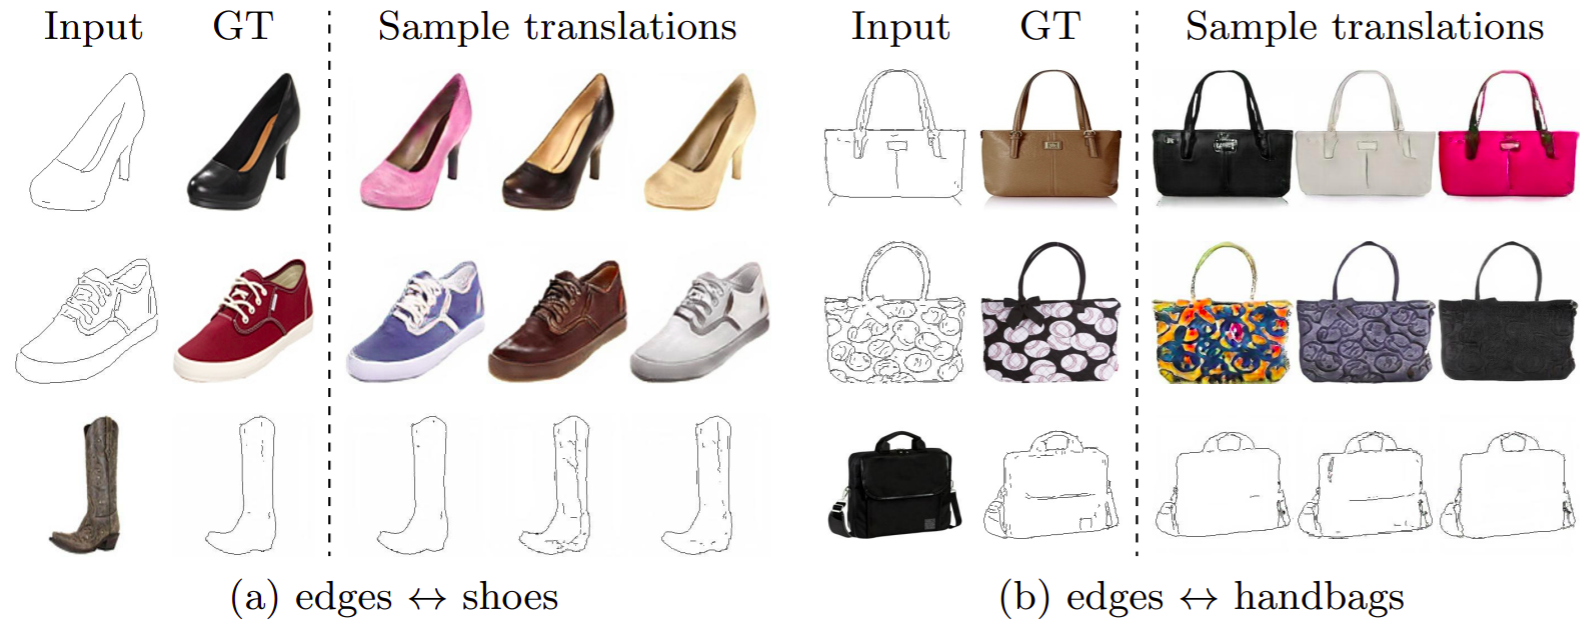
\includegraphics[width=12cm] {images/result_munit_edge.png}
    \caption{Kết quả của MUNIT với bộ dữ liệu Edges and shoes/handbags (Nguồn: \cite{munit})}
    \label{fig:result_munit_edge}
    \end{figure}
    
     \noindent Kết quả đánh giá mô hình MUNIT với bộ dữ liệu Edges and shoes/handbags được trình bày tại Hình \ref{fig:result_munit_edge}. Hình (a) là kết quả chuyển đổi từ ảnh đường nét sang ảnh đôi giày, hình (b) là kết quả chuyển đổi từ ảnh đường nét sang ảnh túi xách. Trong đó, cột đầu tiên là ảnh đầu vào, cột thứ hai là ảnh thực tế, các cột tiếp theo là ảnh sinh ra bởi MUNIT.
    
    \begin{table}[H]
        \label{tab_result}
		\addtolength{\tabcolsep}{8pt}
		\renewcommand\arraystretch{1.3}
		\centering
		\small
		\begin{threeparttable}
			\begin{tabular}{|c|c|c|c|c|c|c|c|}
				\hline
				& \multicolumn{2}{c|}{edges $\rightarrow$ shoes} & \multicolumn{2}{c|}{edges $\rightarrow$ handbags} \\  \cline{2-5}
				& \ Quality\ \  & Diversity &  \ Quality\ \  & Diversity \\
				\hline
				UNIT \cite{unit} & 37.4\% & 0.011 & 37.3\%  & 0.023 \\
				CycleGAN \cite{cycle-gan} & 36.0\% & 0.010 & 40.8\% & 0.012 \\
				MUNIT \cite{munit} & 50.0\% & 0.109 & 50.0\% & 0.175 \\
				BicycleGAN \cite{bicyle-gan} & 56.7\%  & 0.104 & 51.2\% & 0.140 \\
				Real data & N/A & 0.293 & N/A & 0.371 \\
				\hline
			\end{tabular}
			\caption{Kết quả so sánh mô hình MUNIT với các mô hình khác về chất lượng ảnh (Quality) và độ đa dạng của ảnh (Diversity) trên hai bộ dữ liệu edges to shoes và edges to handbags (Nguồn: \cite{munit})}
		\end{threeparttable}
	\end{table}
	
	\noindent Kết quả so sánh mô hình MUNIT với một số mô hình khác trên hai bộ dữ liệu edges to shoes và edges to handbags được trình bày tại bảng trên. Về chất lượng ảnh (Quality), ta sử dụng chỉ số đánh giá bằng con người, còn đối với độ đa dạng của ảnh (Diversity), ta sử dụng chỉ số khoảng cách trung bình LPIPS.

    \begin{figure}[H]
    \centering
    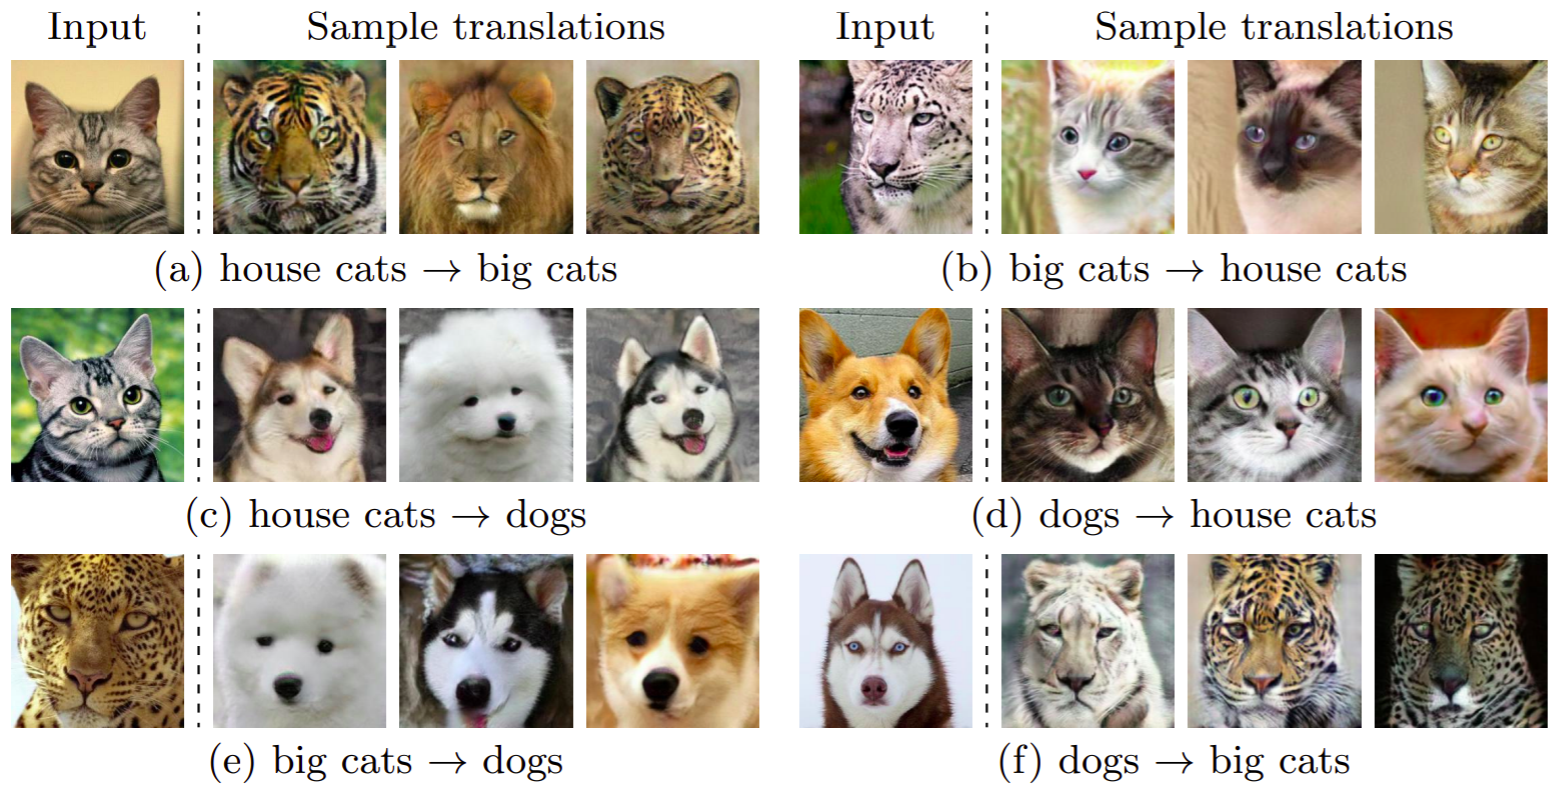
\includegraphics[width=12cm] {images/result_munit_animal.png}
    \caption{Kết quả của MUNIT với bộ dữ liệu Animal image translation (Nguồn: \cite{munit})}
    \label{fig:result_munit_animal}
    \end{figure}
    
     \noindent Hình \ref{fig:result_munit_animal} là kết quả đánh giá mô hình MUNIT với bộ dữ liệu Animal image translation. Các hình từ (a) đến (f) lần lượt là kết quả chuyển đổi của MUNIT với từng cặp dữ liệu từ mèo nhà sang mèo hoang, từ mèo hoang sang mèo nhà, từ mèo nhà sang chó, từ chó sang mèo nhà, từ mèo hoang sang chó, từ chó sang mèo hoang. Trong đó, cột đầu tiên là ảnh đầu vào, các cột sau là kết quả sinh ra bởi MUNIT.

    \begin{figure}[H]
    \centering
    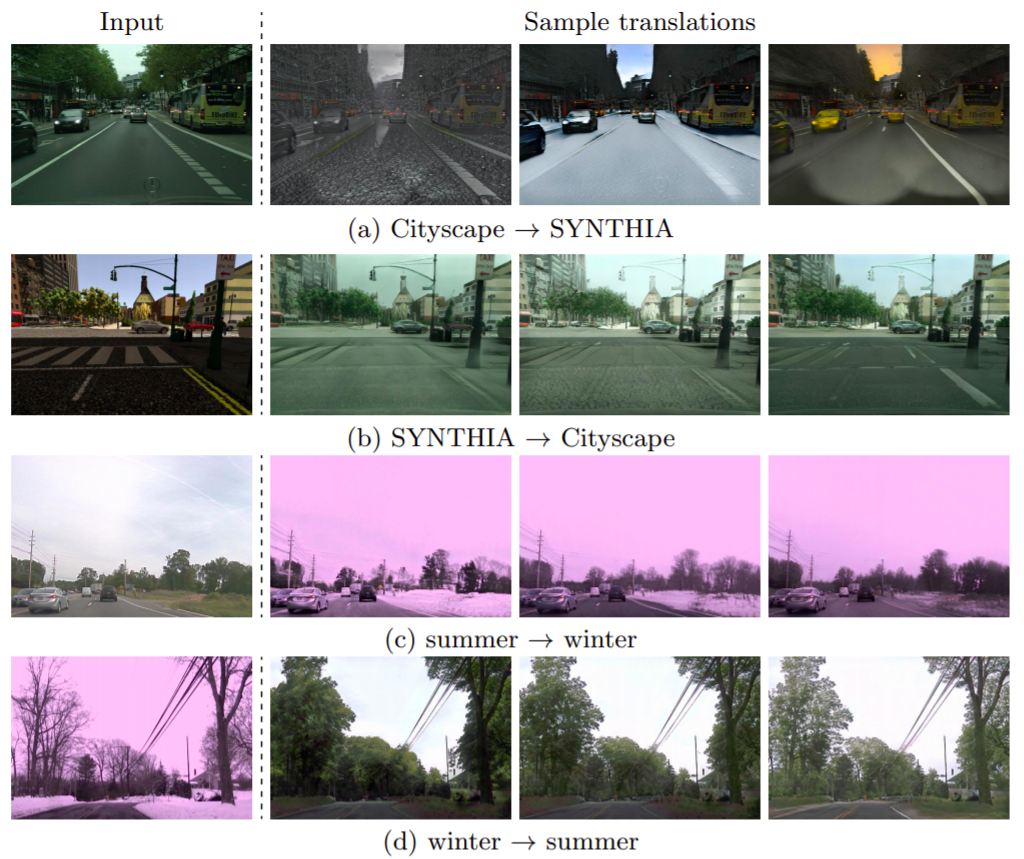
\includegraphics[width=11cm] {images/result_munit_city.png}
    \caption{Kết quả của MUNIT với bộ dữ liệu Street scene images (Nguồn: \cite{munit})}
    \label{fig:result_munit_city}
    \end{figure}

     \noindent Kết quả đánh giá mô hình MUNIT với bộ dữ liệu Street scene images được trình bày tại Hình \ref{fig:result_munit_city}. Các hình từ (a) đến (d) lần lượt là kết quả chuyển đổi của MUNIT với từng cặp dữ liệu từ ảnh Cityscape sang SYNTHIA, từ SYNTHIA sang Cityscape, từ mùa hạ sang mùa đông và từ mùa đông sang mùa hạ. Trong đó, cột đầu tiên là ảnh đầu vào, các cột sau là kết quả sinh ra bởi MUNIT. Trong đó, cột đầu tiên là ảnh đầu vào, cột thứ hai là ảnh thực tế, các cột tiếp theo là ảnh sinh ra bởi MUNIT.

    \begin{figure}[H]
    \centering
    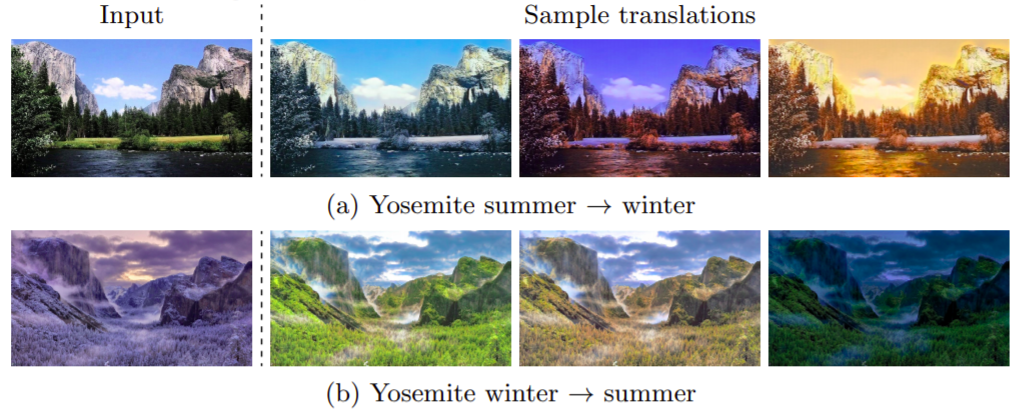
\includegraphics[width=13cm] {images/result_munit_yosemite.png}
    \caption{Kết quả của MUNIT với bộ dữ liệu Yosemite summer and winter (HD) (Nguồn: \cite{munit})}
    \label{fig:result_munit_yosemite}
    \end{figure}
    
     \noindent Kết quả đánh giá mô hình MUNIT với bộ dữ liệu Yosemite summer and winter (HD) được trình bày tại Hình \ref{fig:result_munit_yosemite}. Hình (a) là kết quả chuyển đổi từ ảnh tại Yosemite vào mùa hạ sang mùa đông, hình (b) là kết quả chuyển đổi từ ảnh tại Yosemite vào mùa đông sang mùa hạ. Trong đó, cột đầu tiên là ảnh đầu vào, các cột sau là kết quả sinh ra bởi MUNIT. Trong đó, cột đầu tiên là ảnh đầu vào, cột thứ hai là ảnh thực tế, các cột tiếp theo là ảnh sinh ra bởi MUNIT.

    \begin{figure}[H]
    \centering
    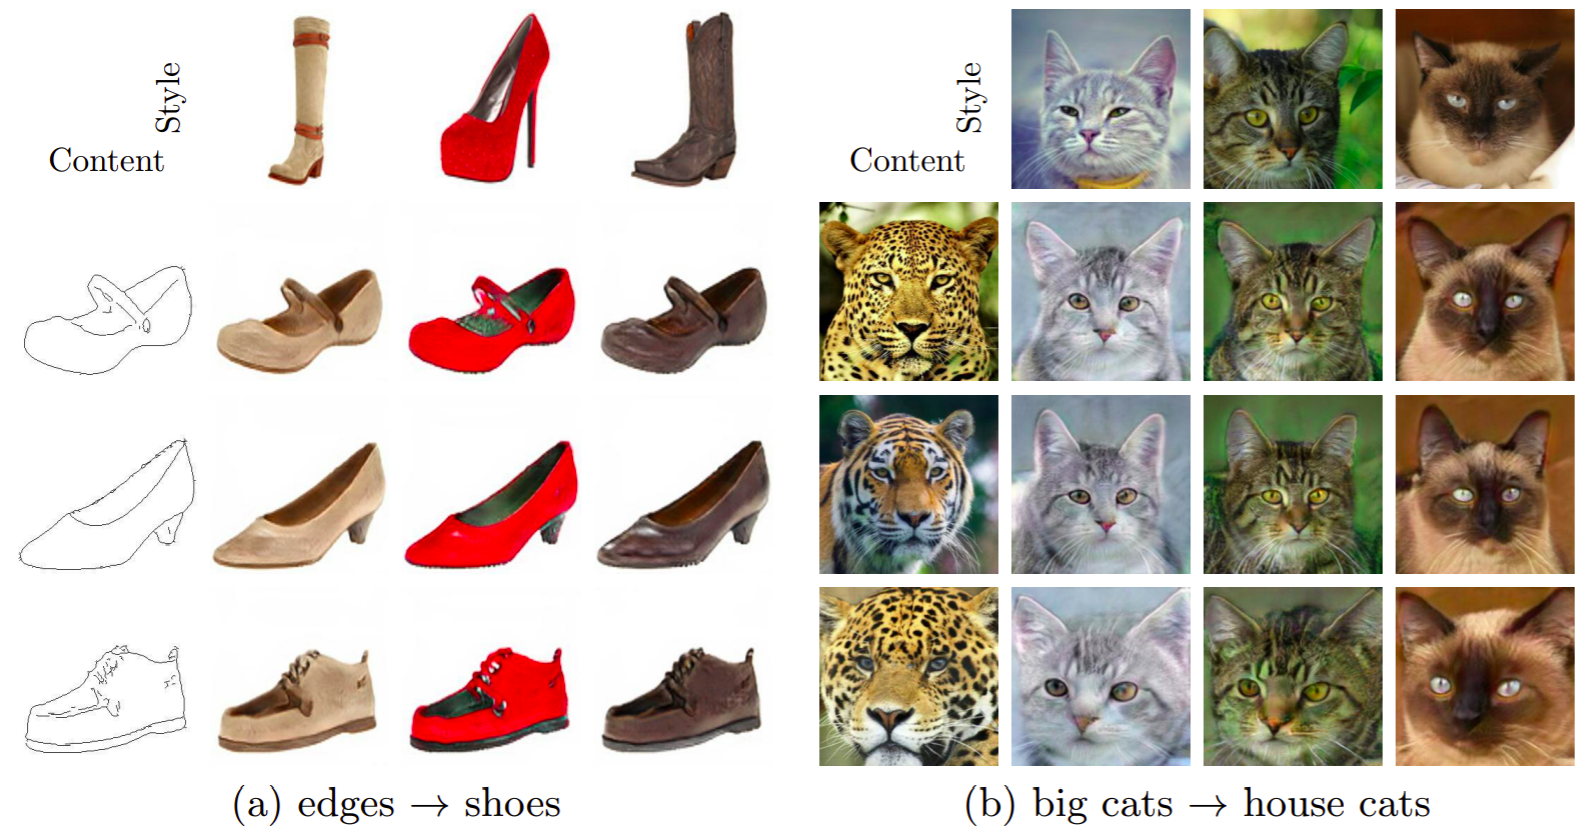
\includegraphics[width=11cm] {images/result_munit_style_transfer.png}
    \caption{Kết quả của MUNIT trong việc xử lý bài toán style transfer (Nguồn: \cite{munit})}
    \label{fig:result_munit_style_transfer}
    \end{figure}
    
    \noindent MUNIT cũng hoạt động rất tốt trong việc giải bài toán style transfer, kết quả được trình bài tại Hình \ref{fig:result_munit_style_transfer}. Hình (a) là kết quả khi chuyển style của ảnh giày sang ảnh đường nét, hình (b) là kết quả khi chuyển style của ảnh mèo nhà sang ảnh mèo hoang. Cột thứ nhất là ảnh đầu vào đóng vai trò là content, hàng thứ nhất là ảnh đầu vào đóng vai trò là style, các ảnh còn lại là kết quả khi kết hợp content và style.
    
    \noindent Hình \ref{fig:result_our_male} và \ref{fig:result_our_female} là kết quả đánh giá mô hình MUNIT với bộ dữ liệu CelebA-HQ. Trong đó, từ trái qua phải, cột thứ nhất và cột thứ ba là ảnh đầu vào, cột thứ hai và cột thứ tư là kết quả sinh ra bởi MUNIT.

    \begin{figure}[H]
    \centering
    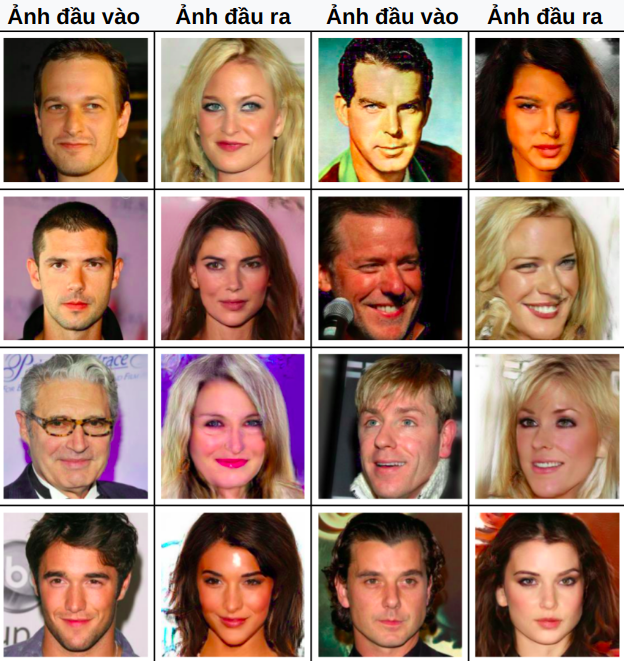
\includegraphics[width=12cm] {images/result_our_male.png}
    \caption{Kết quả của MUNIT trong bài toán biến đổi từ ảnh nam sang ảnh nữ}
    \label{fig:result_our_male}
    \end{figure}
    
    \begin{figure}[H]
    \centering
    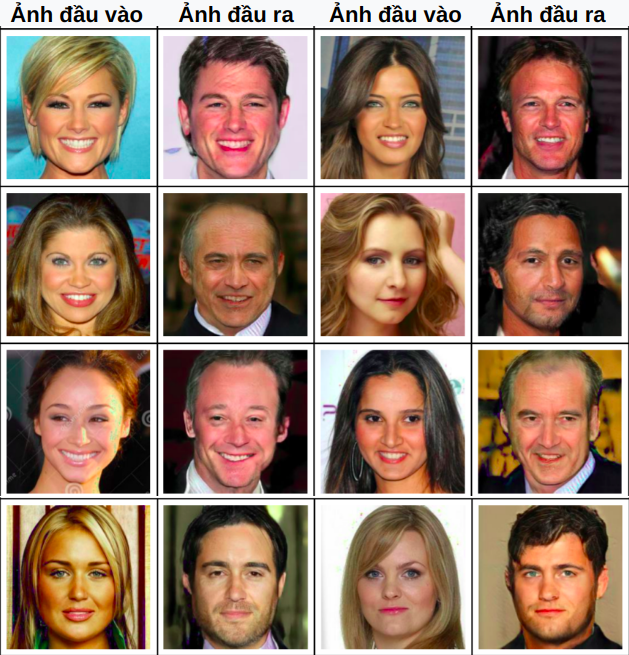
\includegraphics[width=12cm] {images/result_our_female.png}
    \caption{Kết quả của MUNIT trong bài toán biến đổi từ ảnh nữ sang ảnh nam}
    \label{fig:result_our_female}
    \end{figure}
}